\documentclass[twoside, 12pt, a4paper]{article}
%\include{IAP_References.bib}
% List Of Packages
\usepackage{geometry, graphicx, color, fancyhdr, setspace, caption, url}
\usepackage{psfrag,amsbsy,amsmath,textcomp,enumerate}
\usepackage[font=footnotesize]{caption}
\usepackage[nottoc,numbib]{tocbibind}
\usepackage[hidelinks]{hyperref}
\usepackage{multirow}
\usepackage{makecell}
\usepackage{float}
\usepackage{setspace}
\usepackage{notoccite}
\usepackage{longtable}
\usepackage{lscape}
\usepackage{siunitx}
\usepackage{subcaption}
\usepackage{pdflscape}
\usepackage{booktabs}
\usepackage{multicol}
\usepackage{textgreek}
\usepackage[export]{adjustbox}


%\graphicspath{ {./Lab2_Images_Reformatted/} }
%\usepackage{natbib}
% Define Use Of Packages
% Geometry
\geometry{margin = 2.5cm}
\newenvironment{where}{\noindent{}where\begin{itemize}}{\end{itemize}}
\renewcommand{\refname}{REFERENCES}
\renewcommand{\contentsname}{TABLE OF CONTENTS}
%\renewcommand{\listfigurename}{LIST OF FIGURES}
%\renewcommand{\listtablename}{LIST OF TABLES}
% Enter Information
\newenvironment{myindentpar}[1]%
{\begin{list}{}%
		{\setlength{\leftmargin}{#1}}%
		\item[]%
	}
	{\end{list}}

% Fancyhdr
\pagestyle{fancy}
\fancyhead[R]{3803ICT Big Data Analysis, 2022}
\fancyhead[L]{}
\fancyfoot[LE,RO]{\thepage}
\fancyfoot[LO]{Jessy Barber}       % put your names here for fancy footer
\fancyfoot[RE]{Your Title}            % put title here for fancy header
\fancyfoot[C]{}
\renewcommand{\footrulewidth}{0.4pt}

%\bibliographystyle{IEEE}

% Begin The Document
\begin{document}
\begin{titlepage}
\begin{flushright}
	
\includegraphics[height=60px]{griffithlogo.png}
\end{flushright}
\begin{large}
\textbf{Griffith School of Information and Communication Technology}\\
\textbf{Griffith University}

\vspace*{8mm}

\textbf{3803ICT - Big Data Analysis}\\
\textbf{Trimester 1, 2022}
\end{large}

\vspace*{15mm}

\begin{Huge}
\begin{center}
\textbf{Lab Report:}\\
\textbf{Job Market Analysis}
\end{center}
\end{Huge}

\vspace*{5mm}
\begin{large}


\vspace*{8mm}

\textbf{Jessy Barber, s5138877}\\
\hspace*{4.5mm}
\textbf{Zac Jensen, s5153515}\\
\newline

\vspace*{8mm}
\begin{myindentpar}{2cm}
\emph{A report submitted in partial fulfilment of the degree Bachelor of Computer Science}
\end{myindentpar}



\end{large}


\vfill

\end{titlepage}
%-----------------------------------------------------------------------------------------

%next four lines create blank page
%\pagebreak
%\pagestyle{empty}
%\textcolor{white}{This is a blank page}
%\pagebreak

% Contents page

\pagestyle{fancy}
\fancyfoot[C]{\thepage}
\fancyfoot[L,R]{}
\pagenumbering{roman}
\setcounter{page}{1}


%\cleardoublepage
%\phantomsection 

% ----------------------------------------------------------------
\tableofcontents


%\listoffigures
%\listoftables

% ----------------------------------------------------------------
%Document content goes here.
\newpage
\pagenumbering{arabic}
\setcounter{page}{1}
\pagestyle{fancy}

\fancyfoot[LE,RO]{\thepage}
\fancyfoot[LO]{Jessy Barber, s5138877, Zac Jensen, s5153515}                    % insert names for footer here
\fancyfoot[C]{}

\section{Data Preparation and Preprocessing}
The data used in this exploratory analysis will be the provided excel spread sheet, "data.csv". 
\subsection{Describe the Dataset}

\begin{figure}[h]
	\centering
	\includegraphics[scale = 0.65]{cats.png}
	\caption{Categories / Domains of the Dataset}
	\label{fig:cats}
\end{figure}

As seen in figure \ref{fig:cats}, the categories / domains of the dataset are clearly shown. Figure \ref{fig:cats} also shows the number of non-null values that exist in each of these categories. The types of these categories are int64, which represents the lowest salary / highest salary categories, datetime64, which has been used to convert the Date category from its original object format, and the rest of the data are object file formats. The object file format represent strings since these categories contain strings describing their respective job meta data. The original job market dataset contains 13 columns of categories and contains 318'477 rows.\\
This report will conduct multiple vectors of analysis on this job data including analysis on the job metadata / attributes, analysis on the market by locations and analysis on the market by sectors. This analysis will then be visualised using an interactive visualiser. For the attribute analysis, the sector / sub-sectors for each job will be studied, along with the location and range of salaries for each job. The locational analysis will take a further look at the market size in each city and their hottest sectors. The range of salaries common in each city and where the employees are best paid will also be studied. Additionally, the pattern of job posts for each city will be analysed. The market's sectors will then be studied to determine which sectors keep the highest market share, which sub-sectors are of particular interest, what salary ranges are common for each sector / sub-sector, what is the market trend in terms of its sectors and which skills are required for each sector. 

\newpage
\subsection{Describe the Steps You Used for Data Preparation and Preprocessing}

\begin{figure}[h]
	\centering
	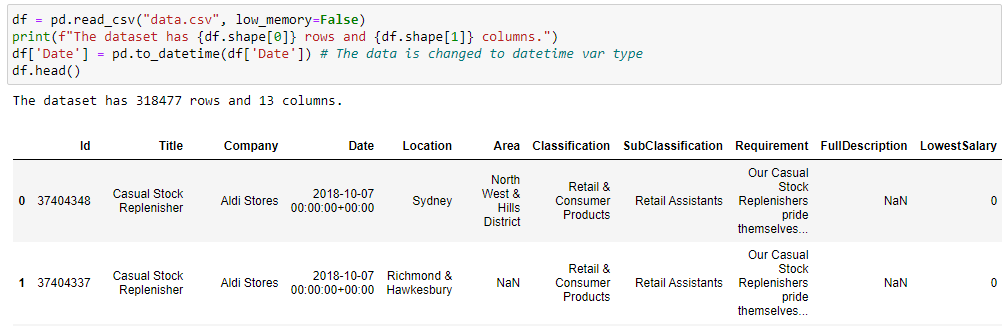
\includegraphics[scale = 0.56]{LoadingDataCode.png}
	\caption{Loading the Data with Pandas}
	\label{fig:LoadingData}
\end{figure}

As seen in figure \ref{fig:LoadingData}, the .csv file is read in and stored as a DataFrame type in the variable df. The head of the dataframe is then printed for visualisation purposes.\\
The first step to begin working with the data is to load it into a DataFrame using Pandas. Pandas is a flexible and powerful open-source data analytics tool, built for use in Python. To load the csv file into a DataFrame, just call read\_csv with the filename. In this assignment, an optional parameter "low\_memory=False" is also provided, to allow Pandas to use enough memory to determine the correct datatype for each column due to the size of the dataset. Without this parameter, Pandas will attempt to guess the datatypes, which may lead to unexpected results. To normalize the data, the average salary is calculated for all job entries, by taking the LowestSalaray and HighestSalary columns, and placed back into the DataFrame as a new column AverageSalary. This number is then multiplied by 1,000 and formatted for easier readabilitiy. This results in an average salary looking like "15,000" instead of "15.0". Normalizing the data this way provides each job entry with a fair visualisation of salary.

The dataset also requires some cleaning for a couple of the columns. The "Id" column is how Seek keeps track of unique job entries and should be an integer number, but occasionally contains some random characters. To clean this up, a regular expression is used to remove any occurence of characters that occur after - and including - an ampersand. The "Date" column also contains extra information that is not necessary for this analysis. This column includes hours, minutes, and seconds, but only the day, month, and year are required. To clean this column, a regular expression is used to remove anything after and including a 'T' character. This results in the "Date" column only containing the necessary information in the format yyyy-mm-dd. After the data cleaning is complete, the correct dtypes are assigned to the "Id" and "Date" columns.

\subsection{Hypothesis About the Analysis Outcome}

One expected outcome of the data analysis is the number of jobs based on location. The expected result is that jobs will be concentrated on the coast, with the highest number seen in the five large cities of Australia. A similar outcome is expected for the salaries of jobs; the further South you go - Melbourne, Sydney, Adelaide - the higher paying jobs you can expect to find. This is due to a large population density and higher cost of living in the Southern cities of Australia.

\newpage 
\section{Data Analysis and Interpretation}
%This section involves performing exploratory analysis, performing statistical analysis and performing predictive analysis on the job market dataset. 
\subsection{Studying the Job Meta Data / Attributes}

\begin{figure}[h]
	\centering
	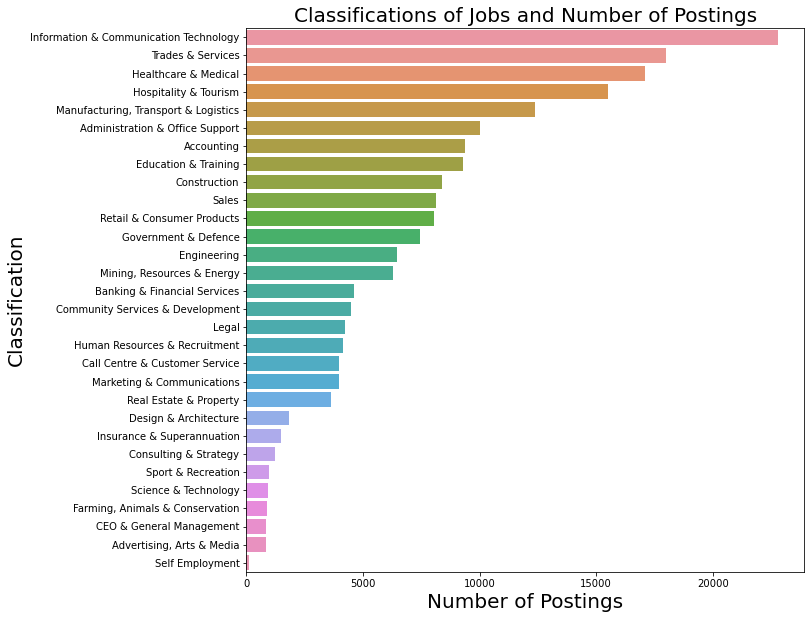
\includegraphics[scale = 0.45]{ClassVsPostings.png}
	\caption{Classification of Jobs and Number of Postings}
	\label{fig:ClassVsPosts}
\end{figure}

\begin{figure}[h!]
	\centering
	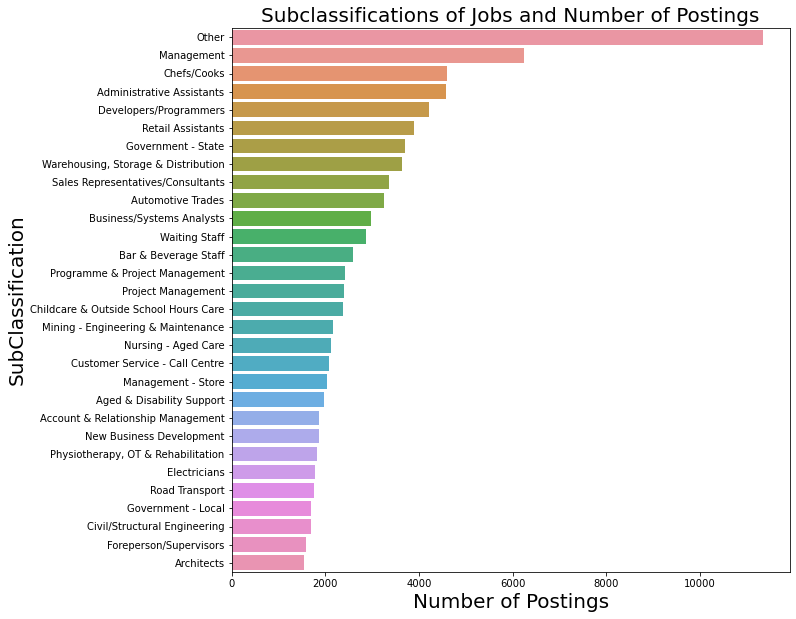
\includegraphics[scale = 0.45]{SubClassVsPostings.png}
	\caption{Subclassification of Jobs and Number of Postings}
	\label{fig:SubClassVsPosts}
\end{figure}

\newpage 
Figure \ref{fig:ClassVsPosts} shows the 30 unique job classifications from the market dataset. Figure \ref{fig:ClassVsPosts} also shows the posting frequency of each of these classifications with information and communication technology, trades and services, healthcare and medical, hospitality and tourism and manufacturing, transport and logistics being in the top five. Figure \ref{fig:SubClassVsPosts} shows the top 30 sub classifications from the market dataset. Figure \ref{fig:SubClassVsPosts} also shows the posting frequency of each of these sub classifications with other, management, chefs / cooks, administrative assistants and developers / programmers being in the top five. 

\begin{figure}[h!]
	\centering
	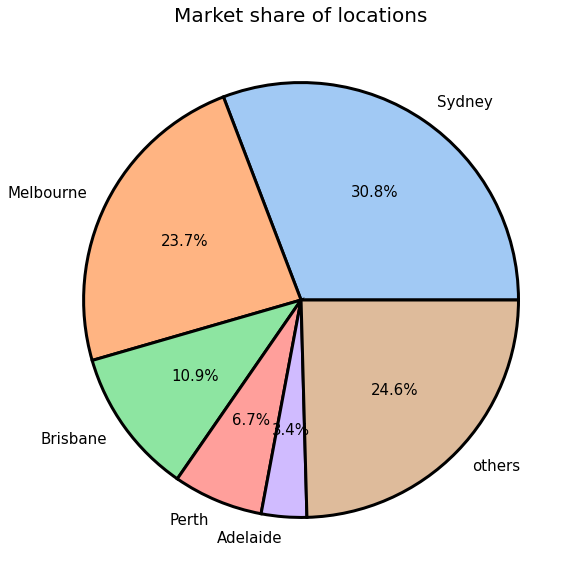
\includegraphics[scale = 0.60]{TopCities.png}
	\caption{Top Five Cities for Market Share}
	\label{fig:TopFiveCities}
\end{figure}

Figure \ref{fig:TopFiveCities} shows the top five cities in Australia in terms of market share from the dataset. It is clear that Sydney holds the highest market share of employment at 30.8\%, Melbourne in second with 23.7\% of the market share and Brisbane in third with 10.9\% of the market share. The other categories represents all other cities in Australia, and accounts for 24.6\% of the market. Adelaide presents the lowest market share at 3.4\% of the top five cities.\\
In the location analysis, the top three cities Sydney, Melbourne and Brisbane will be studied in terms of the market size in each city area, the hottest job sectors, the average salaries and the job posting dates for their respective job listings. 
\newpage
\begin{figure}[h]
	\centering
	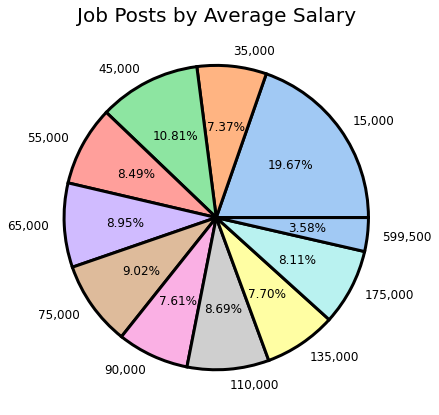
\includegraphics[scale = 0.55]{AverageRanges.png}
	\caption{Average Salary Ranges of Jobs}
	\label{fig:AverageRanges}
\end{figure}

Figure \ref{fig:AverageRanges} shows the average salary range distribution for all of the listed jobs. As seen in this chart, the most common salary is \$15,000 at 19.67\%. Jobs at this salary can expect around \$7.50 per hour working 40 hours a week, 50 weeks a year with 2 weeks of holidays. The highest average salary is around \$599,500 at 3.58\%. Jobs at this salary can expect around \$299.75 per hour working 40 hours a week, 50 weeks a year with 2 weeks of holidays. 

\begin{figure}[h]
	\centering
	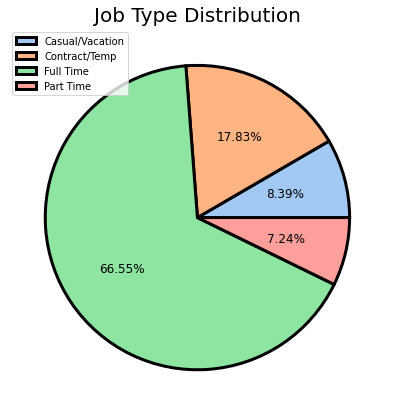
\includegraphics[scale = 0.55]{JobType.png}
	\caption{Distribution of Job Types}
	\label{fig:JobTypes}
\end{figure}

Figure \ref{fig:JobTypes} shows the distribution of advertised job types. From this pie chart it is clear that most jobs are under the job type "Full Time" at 66.55\%, whilst the smallest number of jobs fall under the job type "Part Time" at 7.24\%. 

\newpage
\subsection{Studying the Market by Locations}

\begin{figure}[h!]
	\centering
	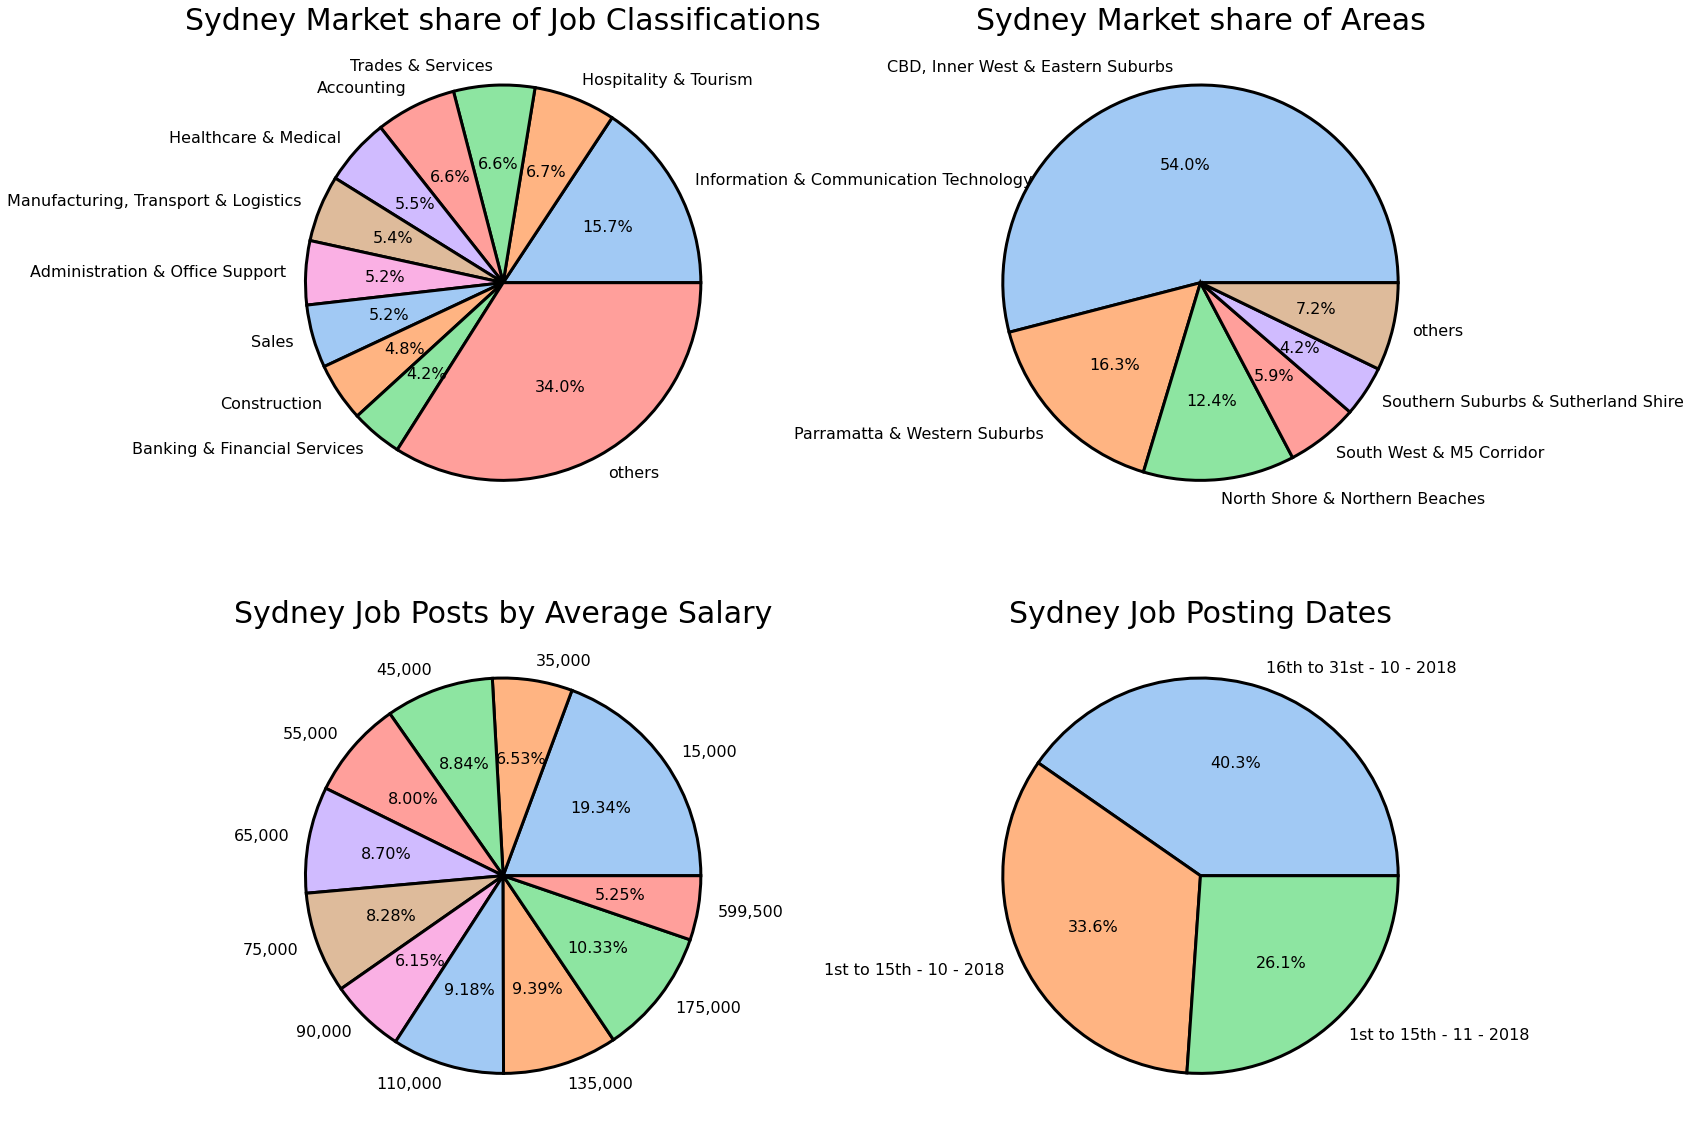
\includegraphics[scale = 0.26]{SydneyLocational.png}
	\caption{Sydney Locational Analysis}
	\label{fig:SydneyLoc}
\end{figure}

\begin{figure}[h!]
	\centering
	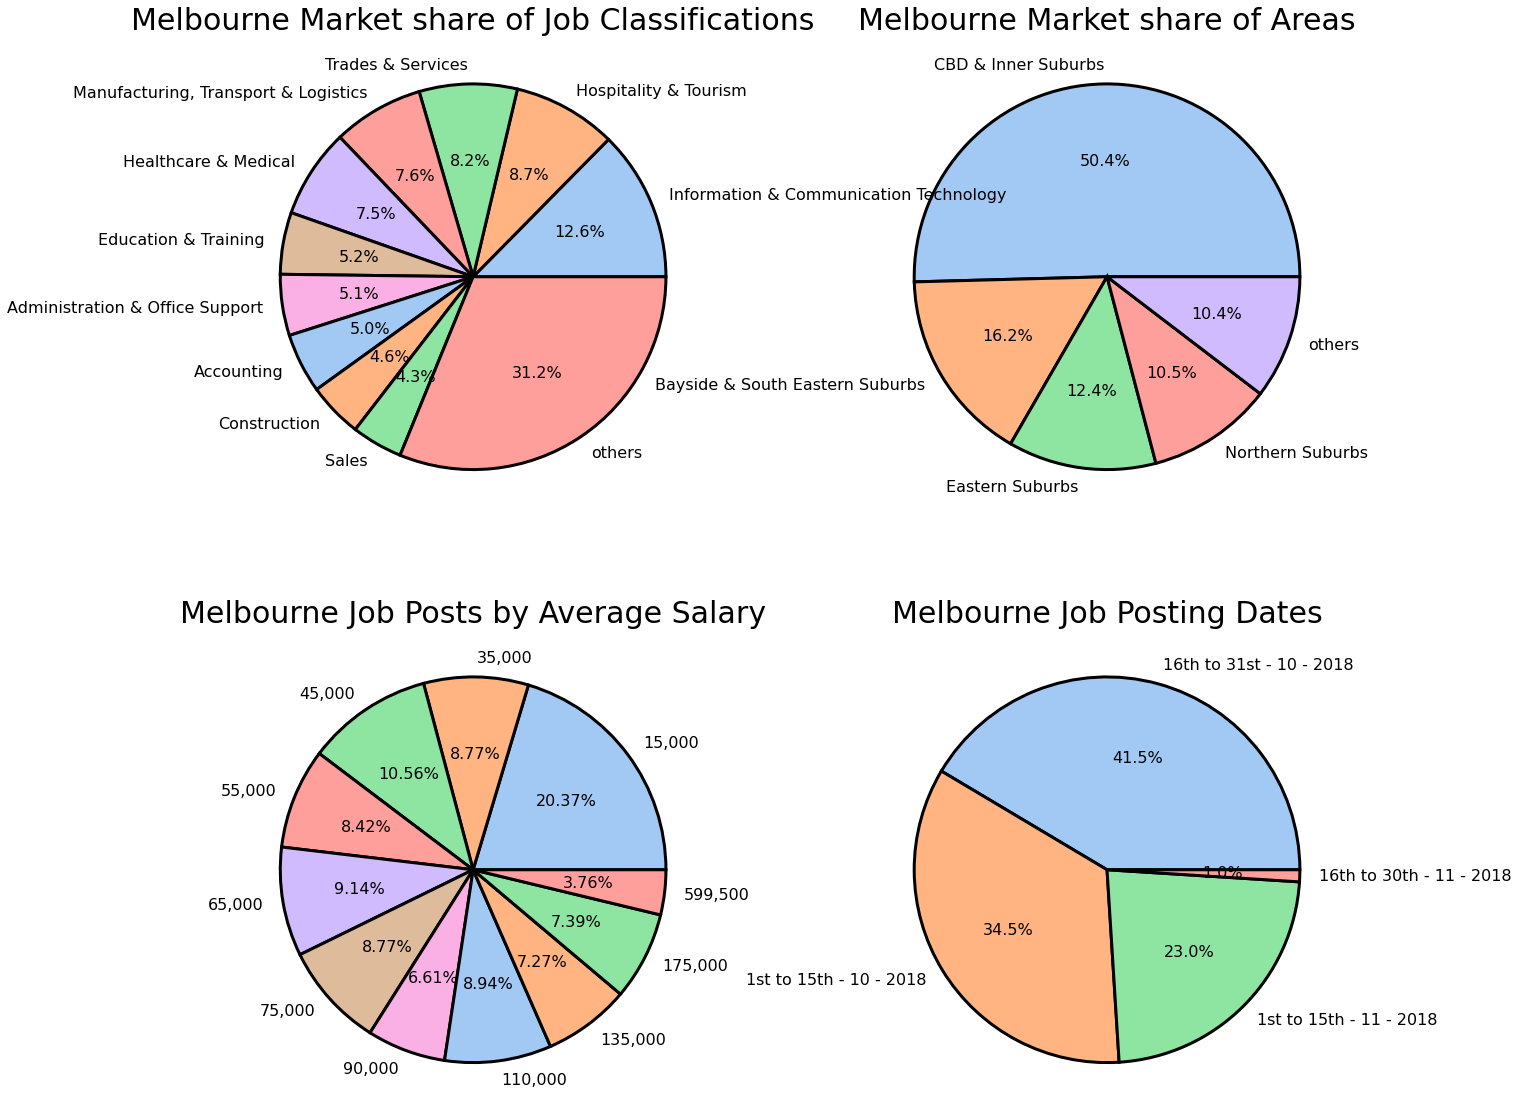
\includegraphics[scale = 0.26]{MelbourneLocational.png}
	\caption{Melbourne Locational Analysis}
	\label{fig:MelbLoc}
\end{figure}

\newpage
\begin{figure}[h]
	\centering
	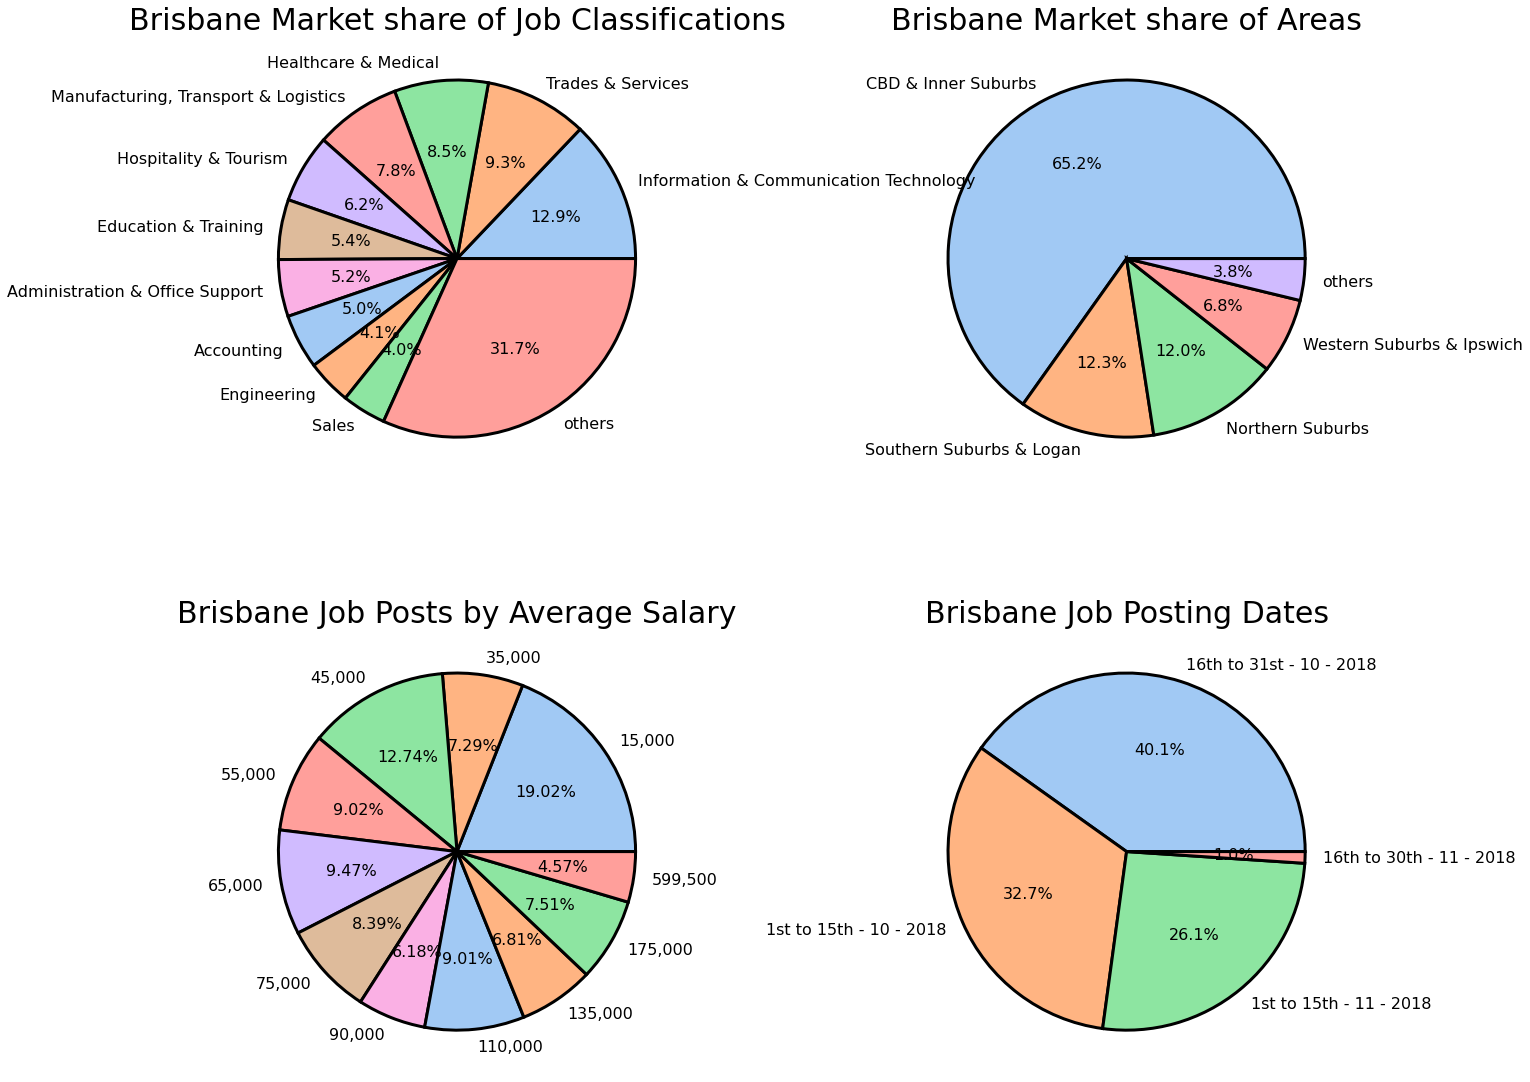
\includegraphics[scale = 0.26]{BrisbaneLocational.png}
	\caption{Brisbane Locational Analysis}
	\label{fig:BrisLoc}
\end{figure}

As seen in figure \ref{fig:SydneyLoc}, the Sydney job market is cornered by the information and communication technology sector which contributes to 15.7\% of the advertised jobs. More than half of the jobs, 54\%, of the market in Sydney are within the CBD, Inner West and Eastern Suburbs. The average salary for the advertised jobs in Sydney is \$15,000 taking up 19.34\%, of the advertised jobs. The least common average salary in Sydney is also the highest at \$599,500 taking up 5.25\% of advertised jobs. The majority of jobs, at 40.3\%, were listed in the second half of October, and 33.6\% and 26.1\% of the jobs were posted in the first half of October and November respectively. The least amount of jobs were advertised in the second half of November at 0\%.\\
As seen in figure \ref{fig:MelbLoc}, the Melbourne job market is also made up with a majority of listings in information and communication technology at 12.6\% of total job listings. The clear majority of job listings in Melbourne are in the CBD and Inner Suburbs of the city. The highest average salary from the job listings in Melbourne is \$15,000 which take up 20.37\% of the advertised jobs. The least common average salary is \$599,500 which consist of 3.76\% of the advertised jobs. Most of the jobs advertised in Melbourne were added in the second half of October at 41.5\% of listings and the first half of October at 34.5\%. The least amount of jobs were listed in the second half of November at 1\%.\\
As seen in figure \ref{fig:BrisLoc}, the highest advertised job in Brisbane is again, information and communication technology at 12.9\% of total job listings. The majority of the advertised jobs in Brisbane are located within the CBD and inner suburbs, accounting for 65.2\% of listings. The average salary in Brisbane is also \$15,000, at 19.02\% of listings, with \$599,500 once again being the least common listed salary at 4.57\% of total listings. Most of the jobs in Brisbane were listen in the second half of October at 40.1\% and the first half of October at 32.7\%. The least amount of jobs were listed in the second half of November at 1\%. 

\newpage
\subsection{Studying the Market by Sectors}

\begin{figure}[h!]
	\centering
	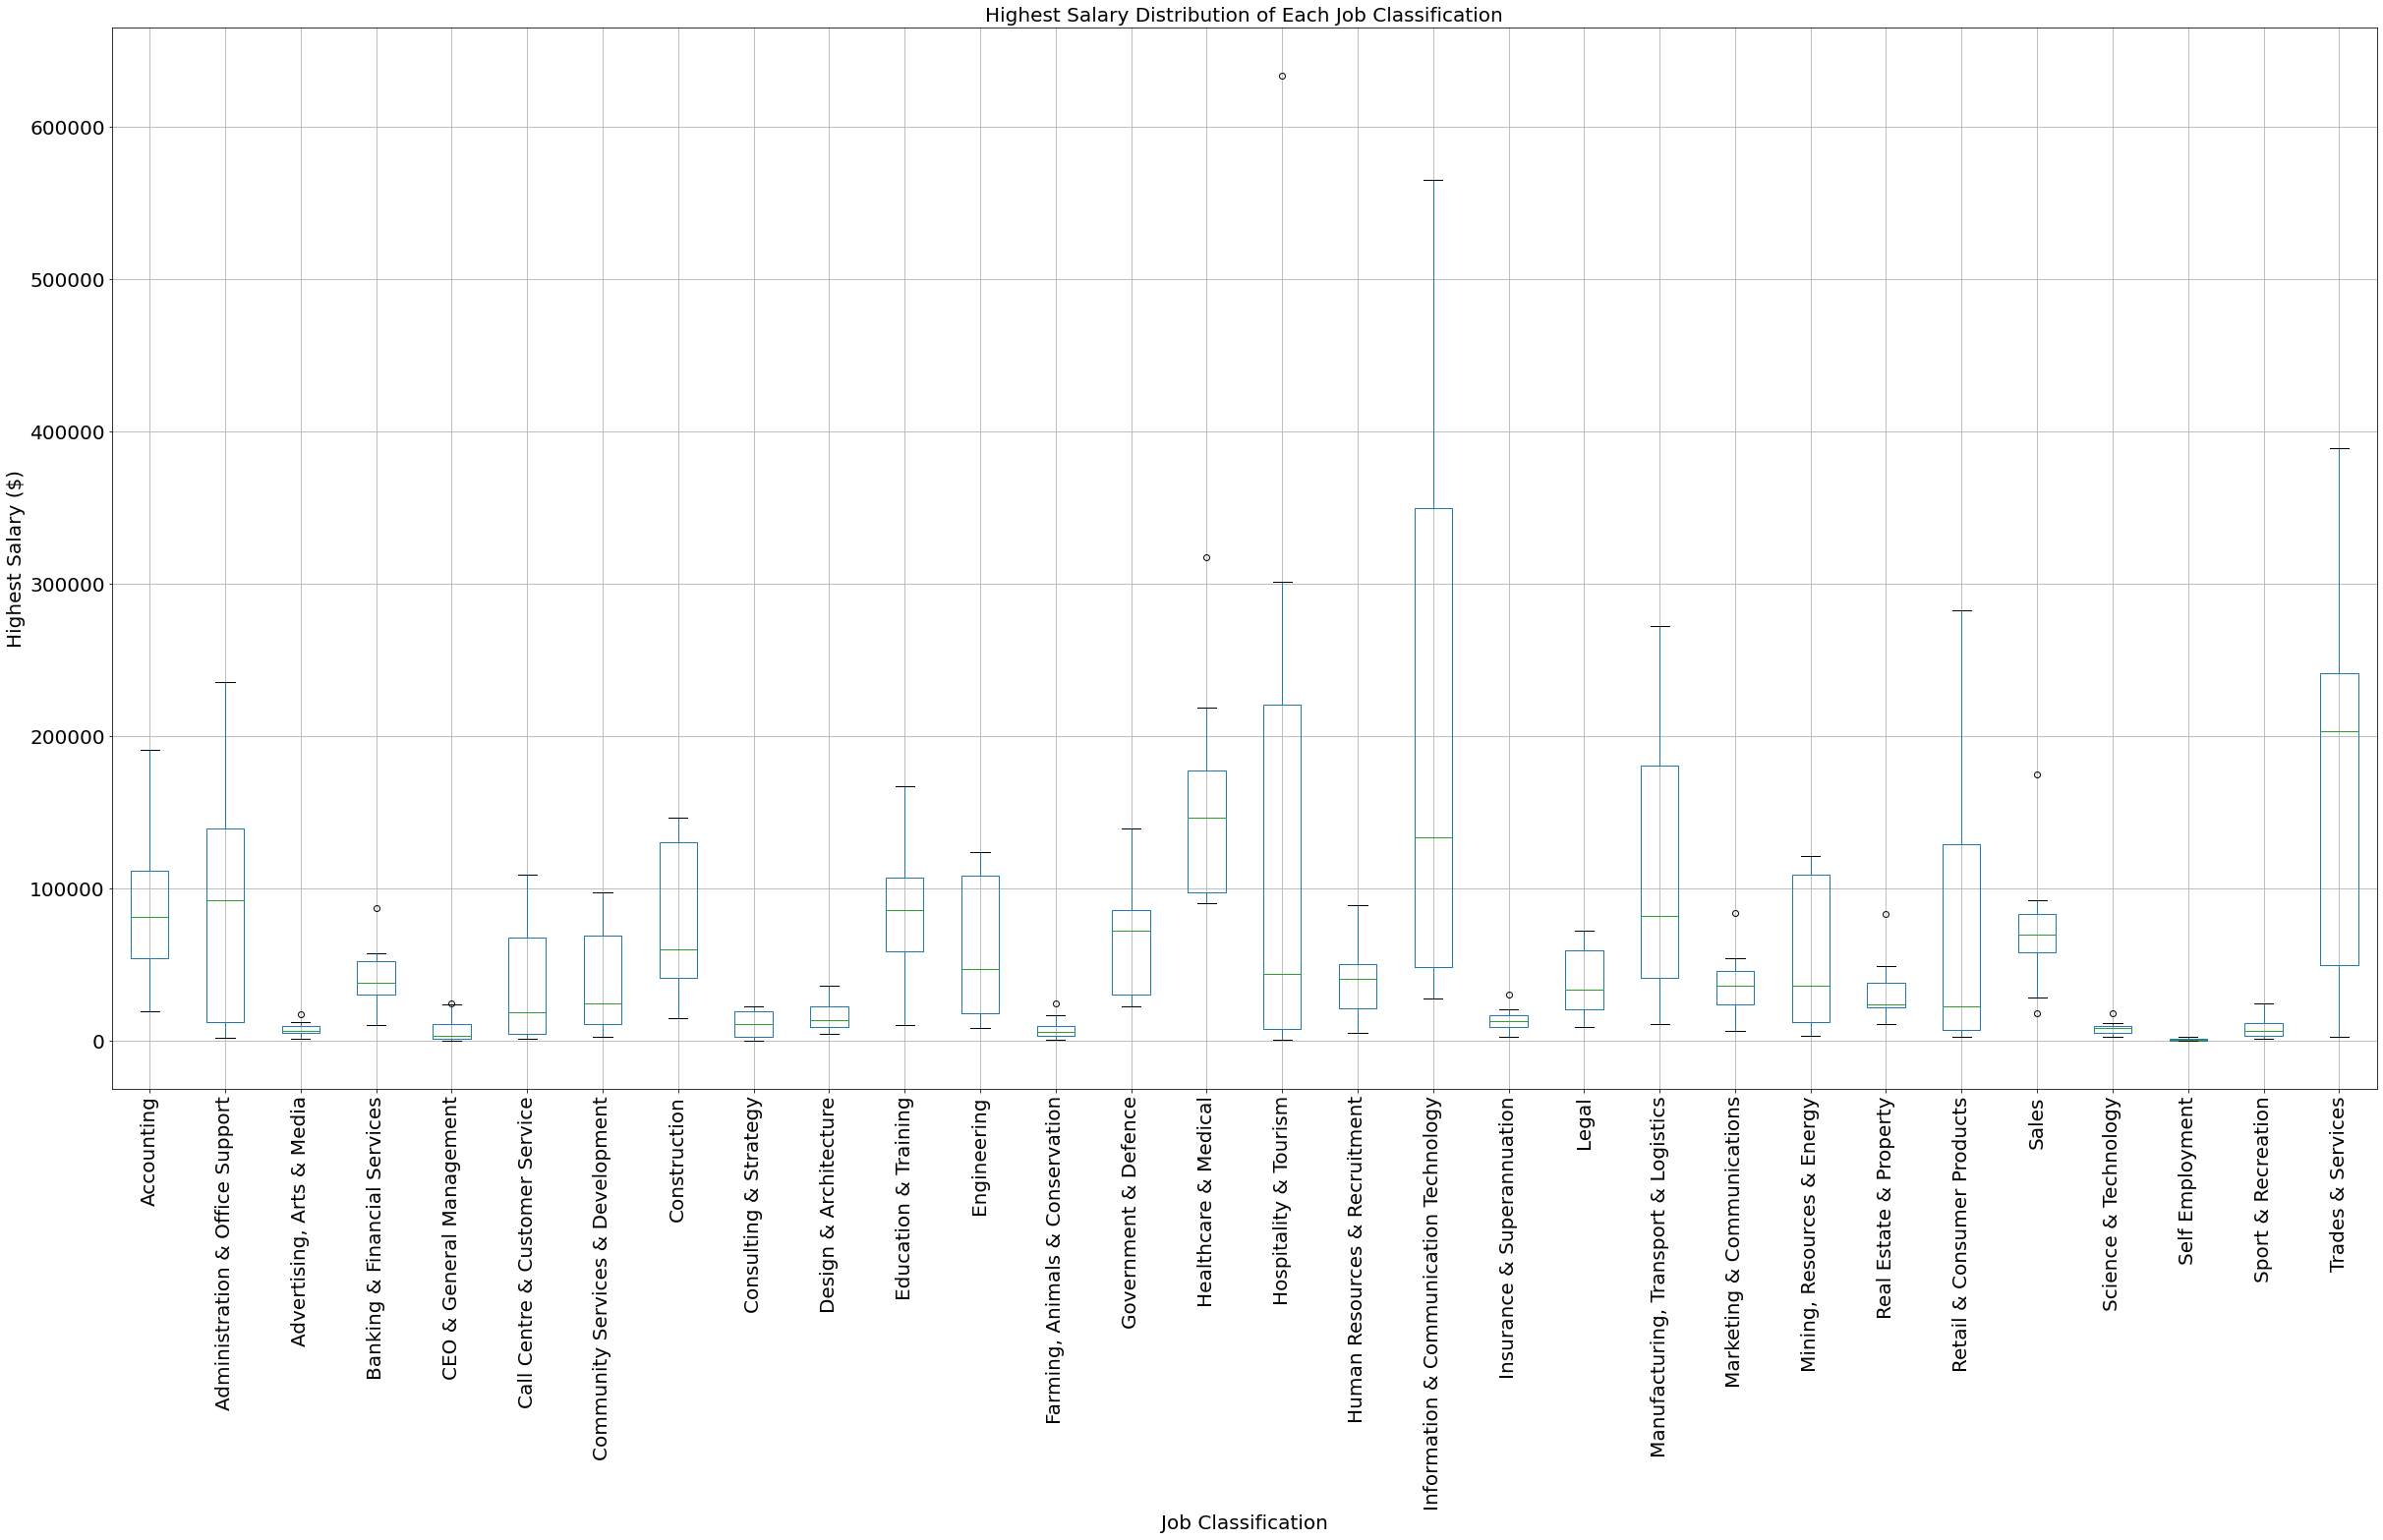
\includegraphics[scale = 0.18]{JobClassHighSal.png}
	\caption{Job Classifications Highest Salaries}
	\label{fig:JobClassHighSal}
\end{figure}

Figure \ref{fig:JobClassHighSal} displays 

\newpage
\subsection{Interactive Visualisation of Results}

\newpage
\section{Evaluation}
\subsection{Findings of Data Analytics}
\subsection{Balancing the Market}
\subsection{Refining the Data Analytics}
\subsection{Implications for Employers and Employees}

\newpage
\section{Case Studies}
\subsection{Case Study 1}
\subsection{Case Study 2}



\end{document}
